
\documentclass[11pt]{article}
\usepackage[utf8]{inputenc}
\usepackage[T1]{fontenc}
\usepackage{geometry}
\geometry{a4paper, margin=1in}
\usepackage{hyperref}
\usepackage{graphicx}
\usepackage{amsmath}
\usepackage{booktabs}
\usepackage{array}
\usepackage{tikz}
\usetikzlibrary{positioning, arrows.meta}

\title{Automating Continuous Household Tidying via Mobile Manipulation\\[2pt]
\large Final-Project Proposal for {\it Robotics}}
\author{Wenbo Ma, Arif Onur Alp, Emir Pisirici\\
RWTH Aachen}
\date{Due: July 11, 2025}

\begin{document}
\maketitle

\begin{abstract}
We present a \textit{PyRoboSim}-based mobile robot that \emph{continuously} tidies a domestic environment by fetching clutter (dirty dishes, laundry, small toys) from their spawning locations and depositing each item in its designated receptacle.  A script-generated PDDL domain captures the pick--navigate--place loop, enabling a symbolic planner to produce high-level task sequences on demand.  Navigation is decomposed into three layers: (i) a global \textbf{RRT*} planner for room-to-room routing; (ii) a real-time grid-based \textbf{A*} planner for local path refinement and(iii) a reactive \textbf{Bug2} controller to escape unforeseen obstacles. Each area in the environment holds a probability score,which is dynamically updated from recent traversals,Objects are classified by a pretrained model, while their locations emerge online through the robot’s continuous exploration. This design lets us focus on navigation, control, and ROS 2 integration without an external perception stack.
\end{abstract}

%-----------------------------------------------------------------
\section{Research Question \& Motivation}

\paragraph{Problem.}
How can a low-cost mobile robot \emph{continuously} locate, collect, and deliver daily clutter---dirty dishes from the living room and soiled laundry from bedrooms---to their appropriate household stations without human supervision?

\paragraph{Relevance.}
Domestic tidying consumes $\approx$1~h/day in the average European home.  Automating the chore improves quality of life and forms a realistic benchmark for service-robot research.

\paragraph{Course linkage.}  Table~\ref{tab:exercises} shows how each of the five lab exercises underpins the proposed system.

\begin{table}[h]
\centering
\begin{tabular}{@{}>{\raggedright}p{1.2cm}>{\raggedright}p{3cm}>{\raggedright\arraybackslash}p{7cm}@{}}
\toprule
\textbf{Ex.} & \textbf{Technique} & \textbf{Role in Project}\\ \midrule
1 & 2-D kinematics, joint chains & Base + 2-DOF arm forward/inverse transforms\\
2 & Sampling motion planning (RRT*) & Global navigation between rooms\\
3 & A*, Bug2 & Local obstacle avoidance and path repair\\
4 & STRIPS / PDDL & Symbolic task sequencing (\textit{collect}$\rightarrow$\textit{drop-off})\\
5 & PyRoboSim/ROS 2 integration & End-to-end execution and monitoring\\ \bottomrule
\end{tabular}
\caption{Pedagogical roots of the project.}
\label{tab:exercises}
\end{table}

%-----------------------------------------------------------------
\section{Proposed Solution}

\subsection{System Architecture}

\begin{figure}[h]
\centering
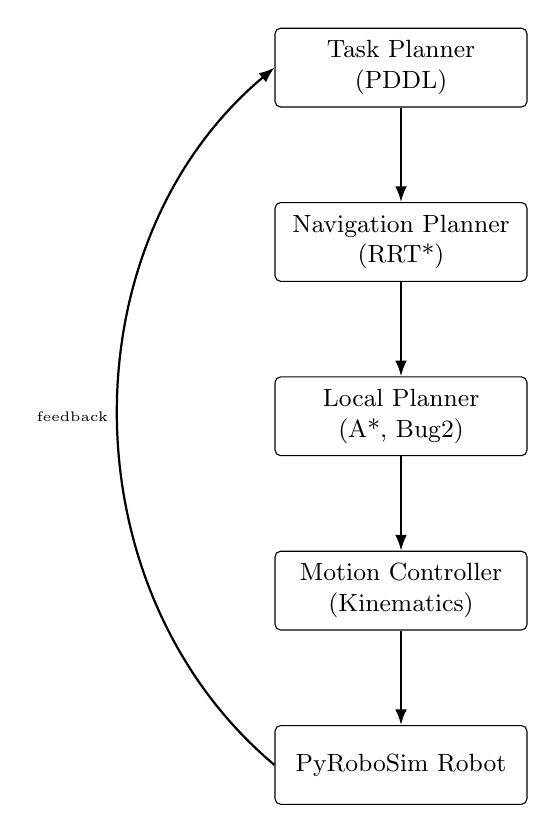
\begin{tikzpicture}[
    node distance = 12mm and 10mm,
    process/.style = {draw, rectangle, rounded corners=2pt,
                      align=center, minimum height=10mm,
                      minimum width=32mm, font=\small},
    arrow/.style = {-{Latex[length=2mm]}, thick}
]
\node[process] (planner) {Task Planner\\(PDDL)};
\node[process, below=of planner] (navg) {Navigation Planner\\(RRT*)};
\node[process, below=of navg] (local) {Local Planner\\(A*, Bug2)};
\node[process, below=of local] (ctrl) {Motion Controller\\(Kinematics)};
\node[process, below=of ctrl] (robot) {PyRoboSim Robot};

\draw[arrow] (planner) -- (navg);
\draw[arrow] (navg) -- (local);
\draw[arrow] (local) -- (ctrl);
\draw[arrow] (ctrl) -- (robot);
\draw[arrow, bend left=50] (robot.west) to node[left, font=\tiny]{feedback} (planner.west);

\end{tikzpicture}
\caption{Layered architecture connecting symbolic planning to execution in PyRoboSim.}
\end{figure}


\begin{description}
\item[World model.]  A PyRoboSim YAML world with rooms, doorways, tables, laundry baskets, and a docking station, augmented by \emph{temporal clutter generators} that spawn dishes/laundry via a Poisson process ($\lambda=1$/5~hour).
\item[Symbolic layer.]  PDDL domain with actions \texttt{navigate}, \texttt{pick}, \texttt{place}, \texttt{dropoff} defined in STRIPS form; plans produced by FastDownward via PyRoboSim's planner API.
\item[Motion layer.]
      \begin{itemize}
        \item \textbf{Global}: RRT* between semantic way-points.
        \item \textbf{Local}: A* on a 0.05~m occupancy grid; Bug2 fallback whenever dynamic obstacles break heuristic guarantees.
      \end{itemize}
\item[Execution monitor.]  ROS~2 action executor.
\item[Continuity.]  A lifecycle node that puts the robot in service every hour.
\end{description}

\subsection{Algorithm--Tool Mapping}

\begin{center}
\begin{tabular}{@{}p{3.3cm}p{4.2cm}p{2cm}@{}}
\toprule
\textbf{Function} & \textbf{Algorithm / Library} & \textbf{Ex.}\\ \midrule
Forward kinematics & Custom Python matrices & 1\\
Global navigation & \texttt{RRT} & 2\\
Local avoidance & \texttt{Bug2/A*}& 3\\
Task planning & \texttt{PDLL, STRIPS} & 4\\
Simulation & PyRoboSim & 5\\ \bottomrule
\end{tabular}
\end{center}

%-----------------------------------------------------------------
\section{Probabilistic Map--Update Example}
\label{sec:example}

We illustrate the belief-map update mechanism with a concise two-frame scenario (Figures~\ref{fig:init_map} and~\ref{fig:adaptive_map}).

\textbf{Frame1 — Initial map.} Figure\ref{fig:init_map} depicts the known world annotated with the robot's \emph{a priori} probability distribution for encountering target objects. Cells shaded \textcolor{red}{red} are searched first, \textcolor{orange}{orange} cells next, and \textcolor{teal}{green} cells last.

\textbf{Frame2 — Experience-driven update.} After one day of operation the robot detects more than ten relevant objects inside a low-priority (green) region. The cell is therefore promoted to \textcolor{orange}{orange} (Figure\ref{fig:adaptive_map}). Analogously, any \textcolor{orange}{orange} cell that accumulates 100+ detections is escalated to \textcolor{red}{red}. This threshold-based adaptation lets the system continuously realign its search strategy with real-world statistics.

\begin{figure}[htbp]
\centering

\includegraphics[width=0.9\linewidth]{second.jpeg}
\caption{Initial probability map with \textcolor{red}{red} = high, \textcolor{orange}{orange} = medium, \textcolor{teal}{green} = low search priority.}
\label{fig:init_map}
\end{figure}

\begin{figure}[htbp]
\centering

\includegraphics[width=0.9\linewidth]{third.jpeg}
\caption{Map after daily update: a previously low-priority region has been promoted to \textcolor{orange}{orange} after 10+ object detections. Regions exceeding 100 detections become \textcolor{red}{red}.}
\label{fig:adaptive_map}
\end{figure}

%-----------------------------------------------------------------
\section{Success Criteria \& Evaluation}
\begin{center}
\begin{tabular}{@{}p{2.8cm}p{3.5cm}p{5cm}@{}}
\toprule
\textbf{Metric} & \textbf{Target} & \textbf{Measurement}\\ \midrule
Task completion & $\ge$90\% items delivered in a service round & Logged world-state queries\\
Planning time & Symbolic $<$ 10s; global path $<$ 5s & ROS~2 timestamps\\
Path optimality & Less then predefined max time & Compare to heuristic bound\\
Git hygiene & $\ge$90\% unit-test coverage; green CI & GitHub Actions\\ \bottomrule
\end{tabular}
\end{center}

A run is \textbf{successful} if all four metrics meet their targets.

%-----------------------------------------------------------------
\section{Project Plan \& Management}

\subsection{Timeline}

\begin{center}
\begin{tabular}{@{}ccl@{}}
\toprule
\textbf{Week} & \textbf{Milestone} & \textbf{Deliverables}\\ \midrule
1 & World-building & YAML house, clutter script\\
2 & Global planner & RRT* node, benchmark notebook\\
3 & Local planner & A* grid \& Bug2, collision tests\\
4 & PDDL domain & STRIPS operators, unit plans\\
5 & Integration & End-to-end demo video\\
6 & Evaluation & Metric harness, stress tests\\
7 & Report \& polish & Final paper, code freeze\\ \bottomrule
\end{tabular}
\end{center}

\subsection{Tools \& Practices}
\begin{itemize}
\item \textbf{Version control:} GitLab, protected \texttt{main}, squash PRs.
\item \textbf{CI:} GitLabActions---lint, pytest, headless simulation, coverage.
\item \textbf{Issue tracking:} GitLab Projects kanban, label taxonomy.
\item \textbf{Docs:} MkDocs auto-deployed to GitLab Pages.
\item \textbf{Risk mitigation:} weekly 20-min review of codes.
\end{itemize}

%-----------------------------------------------------------------
\section{References}

\begin{thebibliography}{8}

\bibitem{LaValle98}
S.\,M.~LaValle, ``Rapidly-Exploring Random Trees: A New Tool for Path Planning,'' 1998.

\bibitem{Fikes71}
R.\,E.~Fikes and N.\,J.~Nilsson, ``STRIPS: A New Approach to the Application of Theorem Proving to Problem Solving,'' \emph{Artificial Intelligence}, 1971.

\bibitem{Hart68}
P.\,E.~Hart, N.\,J.~Nilsson, and B.~Raphael, ``A Formal Basis for the Heuristic Determination of Minimum-Cost Paths,'' \emph{IEEE Transactions on Systems Science and Cybernetics}, 1968.

\bibitem{ChosetBug}
H.~Choset, ``Bug Algorithms,'' CMU Lecture Notes, 2010.

\bibitem{PyRoboSimDoc}
S.~Castro, \emph{pyrobosim}: ROS~2 Enabled 2-D Mobile-Robot Simulator, GitHub, 2025.

\bibitem{PyRoboSimManual}
\emph{PyRoboSim Documentation}, v4.1.0, 2025.

\bibitem{Kavraki96}
L.~Kavraki \emph{et al.}, ``Probabilistic Roadmaps for Path Planning,'' \emph{IEEE Transactions on Robotics and Automation}, 1996.

\bibitem{Robohub22}
Robohub, ``Building a Python Toolbox for Robot Behavior: pyrobosim,'' 2022.

\end{thebibliography}

\end{document}